

%\section{The Concept of Community Clouds}
\section{Community Clouds}
\label{sec:background}

%\subsection{What are community clouds?}
%It is a natural evolution of the growing number of cloud users that within these users certain clusters or communities of users appear,  which can be characterised by shared interest and concerns in cloud computing. 
The wide offer of commercial cloud solutions has led to a widespread adoption of cloud usage by all kinds of stakeholders~\cite{Buyya2011CloudComputing}. 
It is a natural evolution from this growing number of cloud users that within these users, certain clusters or communities of users arise, where each community is characterised by shared interests and common concerns~\cite{Khan2015CommunityClouds}. 
%Cloud communities can extend over several users and they are not necessarily limited geographically. 
%A community however is characterised by having common interests and concerns. 
%For a community cloud to be tailored to a group of users, this group will need to have some specific requirements on the community cloud, different to those of other communities. 
%While communities may be of different size, some kind of critical mass related to this community will be needed to make it worth the effort of developing a tailored community cloud. 
General purpose cloud solutions provided by the public cloud do not optimally fit to the specific needs of the different user communities, since for instance certain security concerns or performance requirements on clouds are only insufficiently addressed by such generic cloud solutions. 
The community cloud solution may have the advantage over the private cloud of sharing the cost of the cloud development and maintenance among its community members. 

%
%This leads to increasing interest in building community cloud solutions which particularly fit to specific communities of users~\cite{Marinos2009}. 
%A community cloud offers features that are tailored to the needs of a specific community. 
%Each community cloud is specialised for providing particular features, the ones which are needed by its community. 
%The difference between one community cloud and another for their users is that the provision of certain features, e.g. performance, security, ease of use of the cloud, are emphasised. 
%
%The specific requirements of a community on its particular cloud will influence the design of the community cloud. 
%While common to community clouds is the concept of addressing the needs of a particular community, its requirements may lead to very different cloud designs between one community cloud and the other. 
%The tailored solutions for each community cloud may affect the hardware needed to build the cloud, the cloud management platforms, the services available in the cloud, and the applications provided to the user community.
%
%The opportunity of community cloud lies in being able to offer optimised cloud solutions to specific user communities. 
%Since cloud user communities can nowadays be identified among the cloud users, drawbacks for them from using off-the-self cloud solutions can be seen, motivating the look at community clouds, since when a community cloud is used, certain requirements of users can be better satisfied. 
%An important condition however is that there is enough commonality between the requirements of the community, e.g. in terms of cloud services that the community uses or cloud performance needs, in order to allow the finding of a specific but common cloud solution. 


%%\subsection{Design Models of Community Cloud}
%Community clouds are implemented using different designs depending upon the requirements, Figure~\ref{fig:cloud_arch} depicts some of these possible architectures. 
%One common approach is that a public cloud provider sets up separate infrastructure and develops services specifically for a community to provide a vertically integrated solution for that market. 
%Similarly, a third party service provider can focus on a particular community and only specialise in building tailor-made solutions for that community.
%Another option is that community members that already have expertise in cloud infrastructures come together to federate their private clouds and collectively provision cloud services to the community. %~\cite{Buyya2010InterCloud}.
%%TODO \minor{}{Citation to [Buyya2010InterCloud] not working!}
%Another radical model involves building community cloud services using resources contributed by individual users by either solely relying on user machines or using them to augment existing cloud infrastructures~\cite{Marinos2009}.
%
%%% FIGURE
%\begin{figure}[tbp]
%   \centering
%   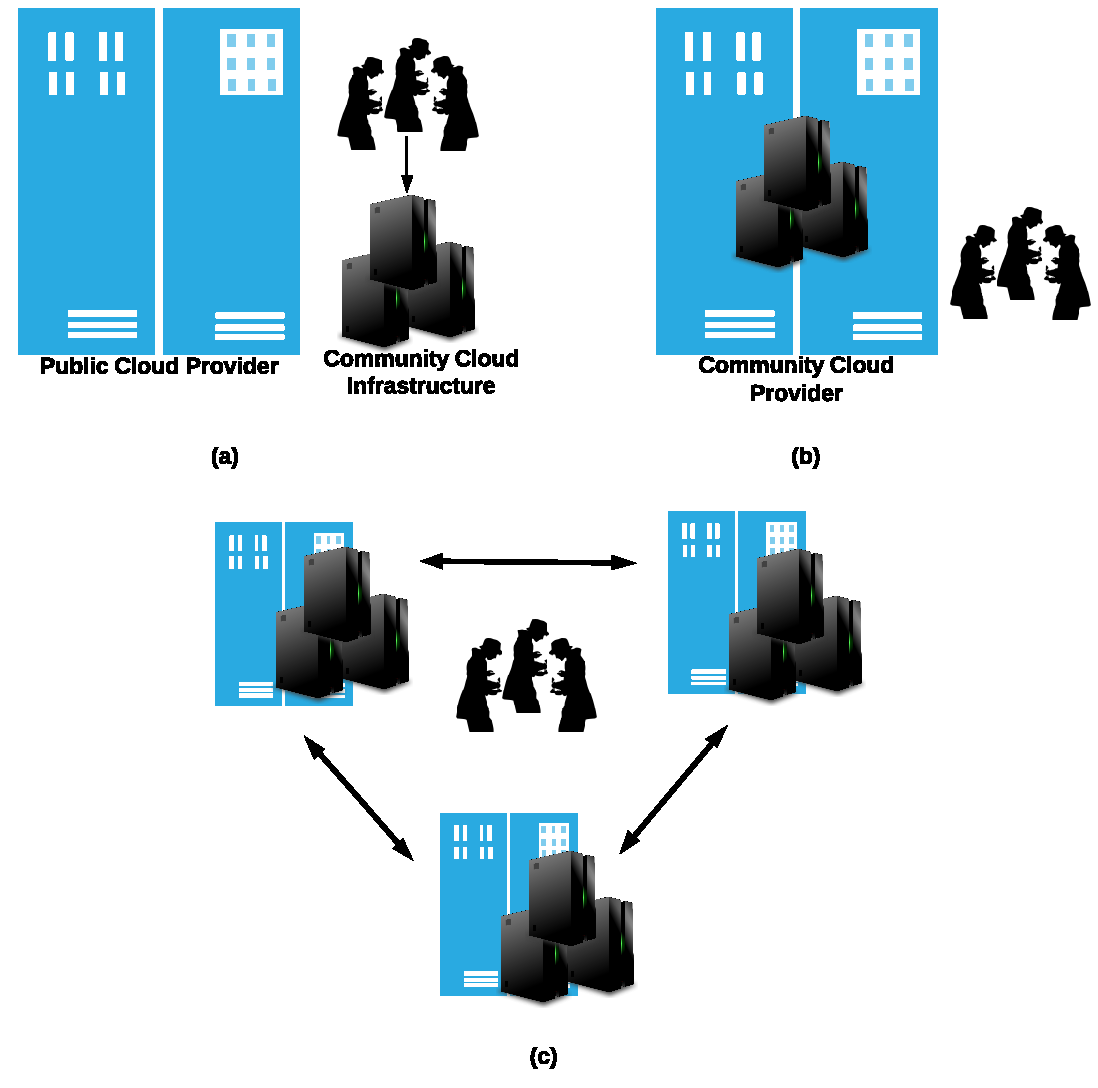
\includegraphics[width=0.5\textwidth,keepaspectratio]{cloud_architecture}
%   \caption{%
%   		Different architectures for community cloud:
%   		(a) Public cloud provider's separate infrastructure for community,
%   		(b) Purpose-built cloud infrastructure for community,
%   		(c) Multiple private clouds combined for community
%   	}
%   \label{fig:cloud_arch}
%\end{figure}
